\section{CapFloor}
\begin{figure}[h]
\centering
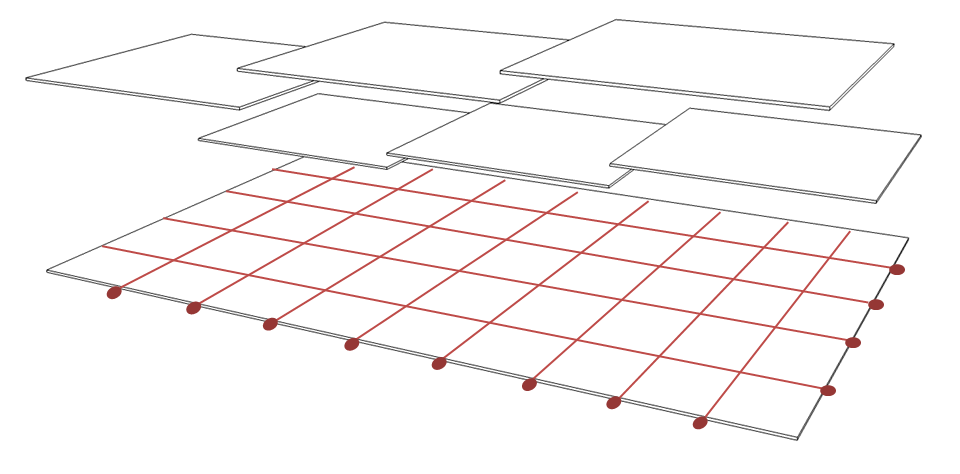
\includegraphics[width=0.8\textwidth]{images/capfloor}
\caption{CapFloor sketch - grid layout of electrodes is placed below a floor layer with sensors attached on the sides}
\label{fig:capfloor_sketch}
\end{figure}

CapFloor is a capacitive system for indoor localization and fall detection that is based on a grid array of sensing electrodes placed below a floor covering \cite{Braun2012CapFloor}. A sketch of the system is shown in Figure \ref{fig:capfloor_sketch}. The grid is comprised of insulated wires that are placed orthogonal to each other. Sensors are placed on two sides of the room. Each sensor is performing loading mode measurements. The system is intended to act as both indoor localization system and fall detector. CapFloor can be placed below any non-conductive material, like wood, tiles and PVC, if the distance between the wires and the floor surface is not too high. It can discriminate between a foot being above an electrode or a whole body. Combining this information from various sensors we are able to get a reliable detection of lying, sitting and standing persons. Using only two sides of the room for sensors it is possible to cut the wires without considerably affecting the signal; allowing easy installation in non-rectangular rooms.
Accordingly CapFloor is able to be used in various application scenarios. Indoor Localization in the home domain can be useful in energy saving and fall prevention by appropriately activating and deactivating the environment lighting. It can also be used in security-restricted areas to detect unauthorized movement. The fall detection should be used in a system that has various levels of escalation. E.g. it is not easy to distinguish between a person doing exercises on a floor and a person that has fallen down. Accordingly the system should query if the person is well and not autonomously call for outside help.
\subsection{Data processing}
Using long wire electrodes may result in considerable noise and influence from outside electric fields. Therefore CapFloor requires preprocessing to reduce the noise and achieve a more robust high-level data processing. The localization uses the weighted average algorithm that has been presented previously. 
\begin{figure}[h]
\centering
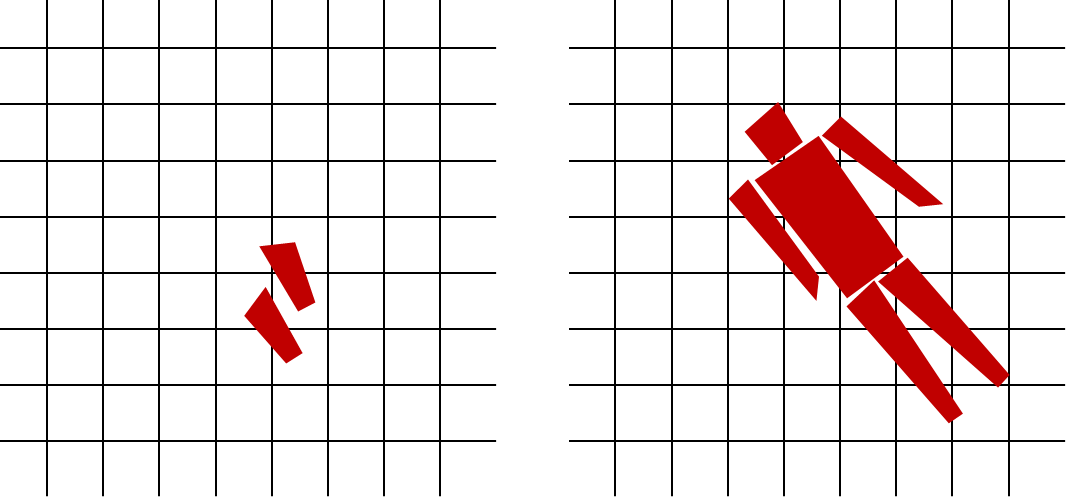
\includegraphics[width=0.8\textwidth]{images/floor_shapes}
\caption{Shapes of a standing and lynig person on top of the CapFloor grid}
\label{fig:capfloor_shapes}
\end{figure}
The fall detection is using a time-series analysis of the aggregated values of the sensors that are currently detecting an object. This method is using the assumption that the overall sensor response is roughly equivalent to the shape of the object that is closest to the surface, resulting in a higher capacitance of the overall system, similar to the plate capacitor model. This effect is shown in Figure \ref{fig:capfloor_shapes}. The sum $s$ of all n sensor values $r$ is the closest equivalent to the system capacitance and therefore a viable measure. If the overall value is beyond a certain threshold $v_l$ we can consider a lying person $p_l$.
\[s=\sum^n_{i=0}{r_i}\ \ \ ,\ \ \ p_l=\left\{ \begin{array}{c}
1,\ \ \ s\ge v_l \\ 
0,\ \ \ s<v_l \end{array}
\right.\] 
In order to increase the robustness this threshold has to be exceeded for a certain amount of time $t_m$. In consequence a fall $f$ is detected if the following equation is 1.
\[f=\prod^{t_m}_{j=0}{p_{l,t_j}}\]
\subsection{Evaluation}
\begin{figure}[h]
\centering
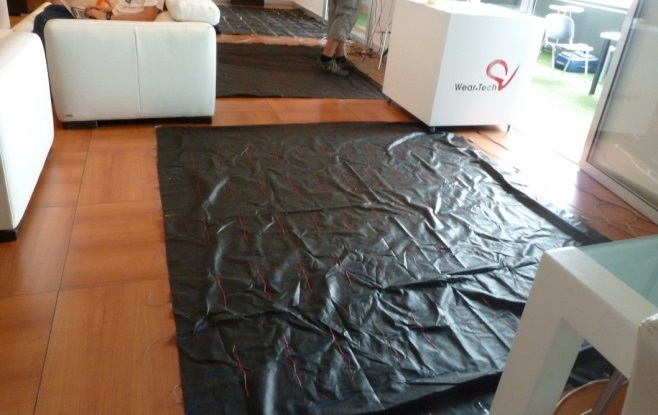
\includegraphics[width=0.8\textwidth]{images/capfloor_evaal}
\caption{Floor mats with integrated CapFloor system used at the EvAAL 2011 competition \cite{Braun2012CapFloor}}
\label{fig:capfloor_evaal}
\end{figure}
The CapFloor system was evaluated in the scope of the Indoor Localization Track of EvAAL 2011, where it participated out of competition \cite{chessa_eval}. In Figure \ref{fig:capfloor_evaal} we can see a picture of the demonstration setup installed in the living lap using the system integrated into different mats that are placed in the environment. The system was tuned to detect a single person and was able to perform this reasonably in the areas covered. The resolution of the system is strongly depending on the given density of electrode wires. While there is a certain measure of proximity, it is not possible to detect objects that are more than a few centimeters away from the wires. Later iterations of the system are using higher voltages and shunt mode measurements to improve the tracking reliability and enhance the fall detection.
